\documentclass{scrreprt}

% Based on the template of Jean-Philippe Eisenbarth:
% - https://github.com/jpeisenbarth/SRS-Tex
% Based on the code of Yiannis Lazarides:
% - http://tex.stackexchange.com/questions/42602/software-requirements-specification-with-latex
% - http://tex.stackexchange.com/users/963/yiannis-lazarides
% Also based on the template of Karl E. Wiegers:
% - http://www.se.rit.edu/~emad/teaching/slides/srs_template_sep14.pdf
% - http://karlwiegers.com

\usepackage{listings}
\usepackage{underscore}
\usepackage[bookmarks=true]{hyperref}
\usepackage[utf8]{inputenc}
\usepackage[english]{babel}
\usepackage{hyperref}
\usepackage{float}
\usepackage{graphicx}

\hypersetup{
    bookmarks=false,                                % show bookmarks bar?
pdftitle={Software Requirement Specification},  % title
pdfauthor={Jean-Philippe Eisenbarth},           % author
pdfsubject={TeX and LaTeX},                     % subject of the document
pdfkeywords={TeX, LaTeX, graphics, images},     % list of keywords
colorlinks=true,                                % false: boxed links; true: colored links
linkcolor=blue,                                 % color of internal links
citecolor=black,                                % color of links to bibliography
filecolor=black,                                % color of file links
urlcolor=black,                                % color of external links
linktoc=page                                    % only page is linked
}

\def\myversion{1.0 }
\date{}
\title{}

\begin{document}


% ----------------------------------------------------------------------------
% Cover
% ----------------------------------------------------------------------------
\begin{flushright}
    \rule{16cm}{5pt}\vskip1cm
    \begin{bfseries}
        \Huge{SOFTWARE REQUIREMENTS\\ SPECIFICATION}\\
        \vspace{1.9cm}
        for\\
        \vspace{1.9cm}
        ICEBERG - LandCover use case\\
        \vspace{1.9cm}
        \LARGE{Version \myversion}\\
        \vspace{1.9cm}
        Prepared by Ioannis Paraskevakos\\
        RADICAL\\
	Brad Spitzbart\\
        Stony Brook University\\
        \vspace{1.9cm}
        \today\\
    \end{bfseries}
\end{flushright}

\tableofcontents


% ----------------------------------------------------------------------------
% Revision History
% ----------------------------------------------------------------------------
\chapter*{Revision History}

\begin{center}
    \begin{tabular}{|c|c|c|c|}
        \hline
        Name & Date & Reason For Changes & Version\\\hline
        Initial & 8/30/2018 & & 0.1\\
        \hline
    \end{tabular}
\end{center}


% ----------------------------------------------------------------------------
% Introduction
% ----------------------------------------------------------------------------
\chapter{Introduction}

\section{Purpose}
The purpose of this document is to capture the requirements of the ICEBERG: Seal
Use Case. It will include functional, non-functional and User Interface requirements.
It will be used as the reference document between the RADICAL Team and the Stony 
Brook team for the Seals use case development.

\section{Document Conventions}
The requested features are listed in section 4 and the non-functional requirements are
listed in section 5. Each of these requirements have a priority from the set {HIGH,
MEDIUM, LOW}. Based on the number of requirements and their priority, a timeline
will be created with each requirement and its expected time-to-completion.

\section{Intended Audience and Reading Suggestions}
%$<$Describe the different types of reader that the document is intended for, 
%such as developers, project managers, marketing staff, users, testers, and 
%documentation writers. Describe what the rest of this SRS contains and how it is 
%organized. Suggest a sequence for reading the document, beginning with the 
%overview sections and proceeding through the sections that are most pertinent to 
%each reader type.$>$

The document is edited and iterated between users and developers. It is intended
to provide the developers as well as the project managers a complete understanding 
of the requirements as they are expected by the users.

An early use case document is provided in [1]. The current status of the project is
provided by the use case Github repository [2].

\section{Project Scope}
\iffalse
$<$Provide a short description of the software being specified and its purpose, 
including relevant benefits, objectives, and goals. Relate the software to 
corporate goals or business strategies. If a separate vision and scope document 
is available, refer to it rather than duplicating its contents here.$>$
\fi
LandCover is 
a pipeline for automated processing of satellite imagery, automated detection and 
removal of snow, ice, water, and shadows from the scene, automated atmospheric 
characterization and removal, and automated ``stretching'' of the scenes to provide
spatial coverage of surveyed area, reasonable estimates on atmospheric contributions, 
and comparisons to a spectral library of known geologic materials.

\section{References}
[1]~\url{https://github.com/iceberg-project/Use-Case-Descriptions/blob/master/LandCover/UseCase_Geology_Draft1_20171101.docx}\newline
[2]~\url{https://github.com/iceberg-project/LandCover}

% ----------------------------------------------------------------------------
% Overall Description
% ----------------------------------------------------------------------------
\chapter{Overall Description}

\section{Product Perspective}
\iffalse
$<$Describe the context and origin of the product being specified in this SRS.  
For example, state whether this product is a follow-on member of a product 
family, a replacement for certain existing systems, or a new, self-contained 
product. If the SRS defines a component of a larger system, relate the 
requirements of the larger system to the functionality of this software and 
identify interfaces between the two. A simple diagram that shows the major 
components of the overall system, subsystem interconnections, and external 
interfaces can be helpful.$>$
\fi
ICEBERG is a multi-disciplinary, cyberinfrastructure, integration project to 
(1) develop open source image classification tools tailored to high-resolution 
satellite imagery of the Arctic and Antarctic to be used on HPDC resources, 
(2) create easy-to-use interfaces to facilitate the development and testing of 
algorithms for application specific geoscience requirements, 
(3) apply these tools through four use cases that span the biological, hydrological, 
and geoscience needs of the polar community, 
(4) transfer these tools to the larger (non-polar) EarthCube community for continued community-driven development.

\section{Product Functions}
\iffalse
$<$Summarize the major functions the product must perform or must let the user 
perform. Details will be provided in Section 3, so only a high level summary 
(such as a bullet list) is needed here. Organize the functions to make them 
understandable to any reader of the SRS. A picture of the major groups of 
related requirements and how they relate, such as a top level data flow diagram 
or object class diagram, is often effective.$>$
\fi

The product functions consist of a series of algorithms to calibrate multispectral 
data from raw digital number through to spectral parameters derived from calibrated 
surface reflectance data.  Intermediate steps include the derivation of top-of-atmosphere 
radiance, the estimation of atmospheric contributions and their removal from the scene, 
the calibration to surface reflectance, the removal of ``non-geological'' surfaces 
(e.g., ice, snow, water, shadow), the parameterization of reflectance data, and the 
``spectral unmixing'' of orbital data using a library of spectral endmembers.

\begin{figure}[H]
 \centering
 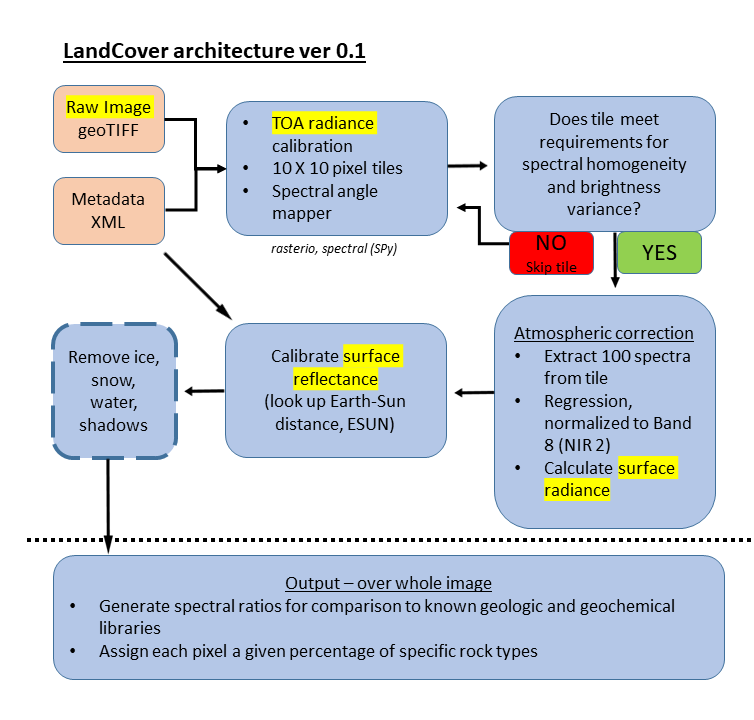
\includegraphics[width=0.8\textwidth]{landcoverarch}
\end{figure}

\section{User Classes and Characteristics}
\iffalse
$<$Identify the various user classes that you anticipate will use this product.  
User classes may be differentiated based on frequency of use, subset of product 
functions used, technical expertise, security or privilege levels, educational 
level, or experience. Describe the pertinent characteristics of each user class.  
Certain requirements may pertain only to certain user classes. Distinguish the 
most important user classes for this product from those who are less important 
to satisfy.$>$
\fi
\begin{itemize}
	\item Community users - web interface
	\item Expert users - local command line interface
	\item Superusers - direct XSEDE interface
\end{itemize}

\section{Operating Environment}
$<$Describe the environment in which the software will operate, including the 
hardware platform, operating system and versions, and any other software 
components or applications with which it must peacefully coexist.$>$

\section{Design and Implementation Constraints}
$<$Describe any items or issues that will limit the options available to the 
developers. These might include: corporate or regulatory policies; hardware 
limitations (timing requirements, memory requirements); interfaces to other 
applications; specific technologies, tools, and databases to be used; parallel 
operations; language requirements; communications protocols; security 
considerations; design conventions or programming standards (for example, if the 
customer’s organization will be responsible for maintaining the delivered 
software).$>$

\section{User Documentation}
\iffalse
$<$List the user documentation components (such as user manuals, on-line help, 
and tutorials) that will be delivered along with the software. Identify any 
known user documentation delivery formats or standards.$>$
\fi
Users will be provided on-line documentation and help.  Syntax, options, and error
messages will be displayed via the web or command line interfaces.

\section{Assumptions and Dependencies}

$<$List any assumed factors (as opposed to known facts) that could affect the 
requirements stated in the SRS. These could include third-party or commercial 
components that you plan to use, issues around the development or operating 
environment, or constraints. The project could be affected if these assumptions 
are incorrect, are not shared, or change. Also identify any dependencies the 
project has on external factors, such as software components that you intend to 
reuse from another project, unless they are already documented elsewhere (for 
example, in the vision and scope document or the project plan).$>$


% ----------------------------------------------------------------------------
% Interface Requirements
% ----------------------------------------------------------------------------
\chapter{External Interface Requirements}

\section{User Interfaces}
$<$Describe the logical characteristics of each interface between the software 
product and the users. This may include sample screen images, any GUI standards 
or product family style guides that are to be followed, screen layout 
constraints, standard buttons and functions (e.g., help) that will appear on 
every screen, keyboard shortcuts, error message display standards, and so on.  
Define the software components for which a user interface is needed. Details of 
the user interface design should be documented in a separate user interface 
specification.$>$

\section{Hardware Interfaces}
%$<$Describe the logical and physical characteristics of each interface between 
%the software product and the hardware components of the system. This may include 
%the supported device types, the nature of the data and control interactions 
%between the software and the hardware, and communication protocols to be 
%used.$>$

The software system requires High Performance Computing (HPC) resources for execution.
The HPC resources should provide CPU and GPU node. Until now, PSC Bridges and SDSC Comet
are the possible candidates.

\section{Software Interfaces}
\iffalse
$<$Describe the connections between this product and other specific software 
components (name and version), including databases, operating systems, tools, 
libraries, and integrated commercial components. Identify the data items or 
messages coming into the system and going out and describe the purpose of each.  
Describe the services needed and the nature of communications. Refer to 
documents that describe detailed application programming interface protocols.  
Identify data that will be shared across software components. If the data 
sharing mechanism must be implemented in a specific way (for example, use of a 
global data area in a multitasking operating system), specify this as an 
implementation constraint.$>$
\fi

The software's middleware should be able to use Unix-based Operating Systems, such as 
Linux and MacOS. The software has library dependencies as listed in Table~\ref{tab:software_dependencies}.
$HARD$ dependency to a library is restricted to the version shown.
$SOFT$ dependency to a library requires as a minimum version the one depicted.


\begin{table}
	\centering
	\begin{tabular}{|c|c|c|}
		\hline
		Library & Version & Type\\\hline
		Python & 3.5 & $SOFT$\\\hline
		matplotlib    & 2.2.2 & $SOFT$ \\\hline
		opencv-python & 3.4.1.15 & $SOFT$ \\\hline
		pandas        & 0.23.0 & $SOFT$ \\\hline
		spectral      & 0.19 & $SOFT$ \\\hline
		xml.etree.ElementTree      &  & $SOFT$ \\\hline
		rasterio  &  & $SOFT$ \\\hline
		\hline
	\end{tabular}
	\caption{Software Dependencies.\label{tab:software_dependencies}}
\end{table}


\section{Communications Interfaces}
$<$Describe the requirements associated with any communications functions 
required by this product, including e-mail, web browser, network server 
communications protocols, electronic forms, and so on. Define any pertinent 
message formatting. Identify any communication standards that will be used, such 
as FTP or HTTP. Specify any communication security or encryption issues, data 
transfer rates, and synchronization mechanisms.$>$


% ----------------------------------------------------------------------------
% Functional Requirements
% ----------------------------------------------------------------------------
\chapter{System Features}
$<$This template illustrates organizing the functional requirements for the 
product by system features, the major services provided by the product. You may 
prefer to organize this section by use case, mode of operation, user class, 
object class, functional hierarchy, or combinations of these, whatever makes the 
most logical sense for your product.$>$

\section{Selecting Parts of the Image for Atmospheric Correction}

\subsection{Description}
As the image is partitioned, each partition is checked whether or not it will be used for the
Atmospheric correction. If yes, it remains to the filesystem, otherwise it is discarded and removed.

\subsection{Stimulus/Response Sequences}
The stimulus is the existence of a partition. The response sequence is if the partition will be kept or not.

\subsection{Functional Requirements}
$<$Itemize the detailed functional requirements associated with this feature.  
These are the software capabilities that must be present in order for the user 
to carry out the services provided by the feature, or to execute the use case.  
Include how the product should respond to anticipated error conditions or 
invalid inputs. Requirements should be concise, complete, unambiguous, 
verifiable, and necessary. Use “TBD” as a placeholder to indicate when necessary 
information is not yet available.$>$

\begin{itemize}
	\item REQ 1:
\end{itemize}


\iffalse
\section{Calibrate to top-of-atmosphere radiance}
%\subsection{Description and Priority}
\subsection{Description}
\iffalse
$<$Provide a short description of the feature and indicate whether it is of 
High, Medium, or Low priority. You could also include specific priority 
component ratings, such as benefit, penalty, cost, and risk (each rated on a 
relative scale from a low of 1 to a high of 9).$>$
\fi
Input multispectral data, calibrate to top-of-atmosphere radiance using ABSCALFACTOR and EFFECTIVEBANDWIDTH parameters 
drawn from image metadata file. 

\subsection{Stimulus/Response Sequences}
$<$List the sequences of user actions and system responses that stimulate the 
behavior defined for this feature. These will correspond to the dialog elements 
associated with use cases.$>$

\subsection{Functional Requirements}
$<$Itemize the detailed functional requirements associated with this feature.  
These are the software capabilities that must be present in order for the user 
to carry out the services provided by the feature, or to execute the use case.  
Include how the product should respond to anticipated error conditions or 
invalid inputs. Requirements should be concise, complete, unambiguous, 
verifiable, and necessary. Use “TBD” as a placeholder to indicate when necessary 
information is not yet available.$>$

$<$Each requirement should be uniquely identified with a sequence number or a 
meaningful tag of some kind.$>$

REQ-1:  REQ-2:

\section{Calculate surface reflectance by automatically applying an atmospheric correction algorithm}
\subsection{Description}
\begin{enumerate}
	\item Identify spectrally homogeneous regions with varying surface illumination 
		and shadowing
	\item Collect ~200 spectra from these locations, ensuring that you are only 
		cataloging variations in brightness (due to illumination) and not variations 
		due to variable surface composition or other chemical/physical properties
	\item Regress a line through these data at each band relative to Band 8, deriving a 
		Y-intercept for each regression, which predicts the radiance value for each 
		band when completely in shadow (attributed solely to atmospheric scattering)
	\item Subtract these Y-intercept values from each image band to calculate surface 
		radiance (atmosphere removed) from top-of-atmosphere radiance
\end{enumerate}


\subsection{Stimulus/Response Sequences}
$<$List the sequences of user actions and system responses that stimulate the 
behavior defined for this feature. These will correspond to the dialog elements 
associated with use cases.$>$

\subsection{Functional Requirements}
$<$Itemize the detailed functional requirements associated with this feature.  
These are the software capabilities that must be present in order for the user 
to carry out the services provided by the feature, or to execute the use case.  
Include how the product should respond to anticipated error conditions or 
invalid inputs. Requirements should be concise, complete, unambiguous, 
verifiable, and necessary. Use “TBD” as a placeholder to indicate when necessary 
information is not yet available.$>$

$<$Each requirement should be uniquely identified with a sequence number or a 
meaningful tag of some kind.$>$

REQ-1:  REQ-2:


\section{Convert to surface reflectance}
\subsection{Description}
Use data from uploaded tables (Earth-Sun distance, ESUN values) to calibrate from surface 
radiance to surface reflectance

\section{Remove non-geological surfaces using derived spectral values (optional)}
\subsection{Description}
\begin{enumerate}
	\item Linearly ``unmix'' the image with a series of spectra from a given library that 
		will include ice, snow, and shadowed and illuminated rock surfaces
	\item Pixels meeting some threshold of non-illuminated geologic rock surfaces will 
		be removed from the scene, leaving behind only illuminated rocky surfaces to be characterized geologically
\end{enumerate}
\textit{OR, a shadow removal method to be determined}

\subsection{Stimulus/Response Sequences}
$<$List the sequences of user actions and system responses that stimulate the 
behavior defined for this feature. These will correspond to the dialog elements 
associated with use cases.$>$

\subsection{Functional Requirements}
$<$Itemize the detailed functional requirements associated with this feature.  
These are the software capabilities that must be present in order for the user 
to carry out the services provided by the feature, or to execute the use case.  
Include how the product should respond to anticipated error conditions or 
invalid inputs. Requirements should be concise, complete, unambiguous, 
verifiable, and necessary. Use “TBD” as a placeholder to indicate when necessary 
information is not yet available.$>$

$<$Each requirement should be uniquely identified with a sequence number or a 
meaningful tag of some kind.$>$

REQ-1:  REQ-2:

\section{Classify land cover geological composition}
\subsection{Description}
\begin{enumerate}
	\item Parameterize spectral data into known parameter mapping products
		
     		\begin{enumerate}
		\item Generate simple spectral ratios and parameter products that 
			can be tied to known geologic and geochemical phenomena
		\item Relative values of these parameters can be used to understand the 
			distribution of mafic compositions, oxidative weathering, and other 
				surface properties
		\end{enumerate}
	\item Linearly ``unmix'' these illuminated geological surfaces using a 
		different endmember library, derived automatically from a library 
		of hundreds of samples based on which library data were derived from 
		a latitude/longitude contained within the scene, assigning each pixel
		a percentage of specifi rock types
\end{enumerate}

\subsection{Stimulus/Response Sequences}
$<$List the sequences of user actions and system responses that stimulate the 
behavior defined for this feature. These will correspond to the dialog elements 
associated with use cases.$>$

\subsection{Functional Requirements}
$<$Itemize the detailed functional requirements associated with this feature.  
These are the software capabilities that must be present in order for the user 
to carry out the services provided by the feature, or to execute the use case.  
Include how the product should respond to anticipated error conditions or 
invalid inputs. Requirements should be concise, complete, unambiguous, 
verifiable, and necessary. Use “TBD” as a placeholder to indicate when necessary 
information is not yet available.$>$

$<$Each requirement should be uniquely identified with a sequence number or a 
meaningful tag of some kind.$>$

REQ-1:  REQ-2:
\fi
% ----------------------------------------------------------------------------
% Nonfunctional Requirements
% ----------------------------------------------------------------------------
\chapter{Other Nonfunctional Requirements}

\section{Performance Requirements}
$<$If there are performance requirements for the product under various 
circumstances, state them here and explain their rationale, to help the 
developers understand the intent and make suitable design choices. Specify the 
timing relationships for real time systems. Make such requirements as specific 
as possible. You may need to state performance requirements for individual 
functional requirements or features.$>$

\section{Safety Requirements}
$<$Specify those requirements that are concerned with possible loss, damage, or 
harm that could result from the use of the product. Define any safeguards or 
actions that must be taken, as well as actions that must be prevented. Refer to 
any external policies or regulations that state safety issues that affect the 
product’s design or use. Define any safety certifications that must be 
satisfied.$>$

\section{Security Requirements}
\iffalse
$<$Specify any requirements regarding security or privacy issues surrounding use 
of the product or protection of the data used or created by the product. Define 
any user identity authentication requirements. Refer to any external policies or 
regulations containing security issues that affect the product. Define any 
security or privacy certifications that must be satisfied.$>$
\fi
All Digital Globe (WorldView) imagery is proprietary and cannot be released publicly. 
Use of imagery must be in accordance with the guidelines and requirements of the Polar 
Geospatial Center and the NGA NextView License. 

\section{Software Quality Attributes}
$<$Specify any additional quality characteristics for the product that will be 
important to either the customers or the developers. Some to consider are: 
adaptability, availability, correctness, flexibility, interoperability, 
maintainability, portability, reliability, reusability, robustness, testability, 
and usability. Write these to be specific, quantitative, and verifiable when 
possible. At the least, clarify the relative preferences for various attributes, 
such as ease of use over ease of learning.$>$

\section{Business Rules}
$<$List any operating principles about the product, such as which individuals or 
roles can perform which functions under specific circumstances. These are not 
functional requirements in themselves, but they may imply certain functional 
requirements to enforce the rules.$>$


% ----------------------------------------------------------------------------
% Other Requirements
% ----------------------------------------------------------------------------
\chapter{Other Requirements}
$<$Define any other requirements not covered elsewhere in the SRS. This might 
include database requirements, internationalization requirements, legal 
requirements, reuse objectives for the project, and so on. Add any new sections 
that are pertinent to the project.$>$


% ----------------------------------------------------------------------------
% Appendixes
% ----------------------------------------------------------------------------
\section{Appendix A: Glossary}
%see https://en.wikibooks.org/wiki/LaTeX/Glossary
$<$Define all the terms necessary to properly interpret the SRS, including 
acronyms and abbreviations. You may wish to build a separate glossary that spans 
multiple projects or the entire organization, and just include terms specific to 
a single project in each SRS.$>$

\section{Appendix B: Analysis Models}
$<$Optionally, include any pertinent analysis models, such as data flow 
diagrams, class diagrams, state-transition diagrams, or entity-relationship 
diagrams.$>$

\section{Appendix C: To Be Determined List}
$<$Collect a numbered list of the TBD (to be determined) references that remain 
in the SRS so they can be tracked to closure.$>$

\end{document}

